% ============================================================
% A1 research poster (DIN A1 portrait, 594 x 841 mm)
% Theme: Gemini (MIT licence) - https://github.com/anishathalye/gemini
% Compile with:  xelatex poster.tex   (needs the Lato font)
% All reported numbers come from results/results.json (see the repository).
% ============================================================
\documentclass[final]{beamer}

\usepackage[size=custom,width=59.4,height=84.1,scale=1.0]{beamerposter}
\usetheme{gemini}
\usecolortheme{gemini}
\usepackage{graphicx}
\usepackage{booktabs}
\usepackage{tabularx}
\usepackage{amsmath}
\usepackage{tikz}
\usetikzlibrary{arrows.meta,positioning}

% ---------- Font sizes (exam rule: text >= 24 pt; \normalsize = 24.88 pt) ----------
\setbeamerfont{headline title}{size=\huge,series=\bfseries}
\setbeamerfont{headline author}{size=\large}
\setbeamerfont{headline institute}{size=\large}
\setbeamerfont{block title}{size=\LARGE}
\setbeamerfont{caption}{size=\normalsize}

% ---------- Colours ----------
\definecolor{navy}{RGB}{39,60,117}
\definecolor{steel}{RGB}{64,115,158}
\definecolor{paleblue}{RGB}{232,240,250}
\definecolor{wm}{RGB}{243,243,243}
\setbeamercolor{headline}{fg=white,bg=navy}
\setbeamercolor{headline rule}{bg=steel}
\setbeamercolor{block title}{fg=navy,bg=white}
\setbeamercolor{block separator}{bg=navy}
\setbeamercolor{block title alerted}{fg=navy,bg=paleblue}
\setbeamercolor{block separator alerted}{bg=navy}
\setbeamercolor{block body alerted}{fg=black,bg=paleblue}
\setbeamercolor{caption name}{fg=navy}
\definecolor{lightgrey}{RGB}{244,245,247}
\setbeamercolor{block title example}{fg=navy,bg=lightgrey}
\setbeamercolor{block separator example}{bg=navy}
\setbeamercolor{block body example}{fg=black,bg=lightgrey}
\newenvironment{keyblock}[1]{%
  \setbeamercolor{block title alerted}{fg=white,bg=navy}%
  \setbeamercolor{block separator alerted}{bg=white}%
  \setbeamercolor{block body alerted}{fg=white,bg=navy}%
  \begin{alertblock}{#1}}{\end{alertblock}}


% ---------- Layout ----------
\newlength{\sepwidth}
\newlength{\colwidth}
\setlength{\sepwidth}{0.03\paperwidth}
\setlength{\colwidth}{0.2933\paperwidth}
\newcommand{\separatorcolumn}{\begin{column}{\sepwidth}\end{column}}
\newcommand{\hyp}[2]{\textbf{\color{navy}#1}\enspace #2\par}
\newcommand{\bibent}[2]{\makebox[1.6em][l]{[#1]}#2\par}

% ---------- Title ----------
\title{Not Bad, Not Good?\\Sentiment Models under Negation}
\author{Priyadith Hosahalli Nagesh \quad·\quad Vismaya Basavaraju Mamatha}
\institute{Trends in Natural Language Processing \quad·\quad SoSe 2026}

% University logo: put the official file next to poster.tex as logo_unitrier.png (or .pdf).
% A white/negative version works best on the navy header.
% Official Universitaet Trier logo, set on a white panel to match the QR panel.
% Height 3.5cm -> approx 14.4cm wide at ~230 PPI (exam rule: figures >= 150 PPI).
\IfFileExists{logo_unitrier.pdf}{\logoleft{\fcolorbox{white}{white}{\includegraphics[height=3.0cm]{logo_unitrier.pdf}}}}{%
\IfFileExists{logo_unitrier.png}{\logoleft{\fcolorbox{white}{white}{
\includegraphics[height=3.0cm]{logo_unitrier.png}}}}{%
\logoleft{}}}
\logoright{\IfFileExists{qr_repo.png}{\fcolorbox{white}{white}{
\includegraphics[height=6.1cm]{qr_repo.png}}}{\fcolorbox{white}{navy}{\parbox[c][6.5cm][c]{6.5cm}{\centering\color{white}\fontsize{30}{38}\selectfont QR code\\to repository}}}}

\footercontent{%
  github.com/PriyadithGowda/negation-sentiment \hfill
  Full reference list in the appendix}

\begin{document}
\begin{frame}[t]
\begin{columns}[t]
\separatorcolumn

% ==================== COLUMN 1: HYPOTHESIS ====================
\begin{column}{\colwidth}

\begin{block}{1 \textbullet{} Hypothesis}
\heading{Motivation}
On the SST-2 benchmark~[5], the fine-tuned RoBERTa model tested here labels \textbf{every} one of our unmodified seed sentences correctly. Yet a single operator such as \emph{not}, \emph{but} or \emph{very} can reverse or weaken the polarity of a sentence while leaving most words unchanged.

Language models are known to struggle with negation~[2,\,3,\,6], and behavioural testing reveals failures that held-out accuracy hides~[1]. This poster puts three model families on the \textbf{same minimal pairs} and checks the findings against \textbf{naturally occurring} negation.
\end{block}

\begin{alertblock}{Research Questions}
\hyp{RQ1}{How robust are lexicon-based, fine-tuned and instruction-tuned models to polarity-changing operators?}
\hyp{RQ2}{Which linguistic phenomena cause the most errors?}
\hyp{RQ3}{Does benchmark accuracy predict robustness?}
\end{alertblock}

\begin{block}{Hypotheses}
\hyp{H1}{The lexicon-based VADER~[4] has the highest error rates, since its negation rule only inspects a fixed three-word window.}
\hyp{H2}{Fine-tuned RoBERTa handles simple negation but fails on double negation.}
\hyp{H3}{The instruction-tuned LLM is the most robust model across all phenomena.}
\end{block}

\begin{block}{Contribution}
A \textbf{controlled comparison of lexicon-based, fine-tuned and instruction-tuned models on one validated minimal-pair suite covering five negation phenomena}, checked against natural SST-2 negation and backed by a quantified error taxonomy.
\end{block}


\end{column}
\separatorcolumn

% ==================== COLUMN 2: METHODOLOGY ====================
\begin{column}{\colwidth}

\begin{block}{2 \textbullet{} Methodology}
\heading{Test suite construction}
\begin{center}
\begin{tikzpicture}[
  box/.style={draw=navy,line width=2pt,fill=paleblue,rounded corners=6pt,
              text width=4.4cm,inner sep=4pt,minimum height=3.8cm,align=center},
  arr/.style={-{Latex[length=6mm,width=5mm]},line width=2.5pt,navy}]
  \node[box] (a) {\textbf{Seed}\\44 SST-2\\sentences};
  \node[box,right=0.95cm of a] (b) {\textbf{Perturb}\\5 types\\219 items};
  \node[box,right=0.95cm of b] (c) {\textbf{Validate}\\2 raters\\$\kappa = 1.00$};
  \draw[arr] (a) -- (b);
  \draw[arr] (b) -- (c);
\end{tikzpicture}
\end{center}

\begin{table}
\begin{tabularx}{\linewidth}{@{}lXc@{}}
\toprule
\textbf{Phenomenon} & \textbf{Example} & \textbf{Gold}\\
\midrule
Seed          & \emph{The food was good.}              & pos\\
Negation      & \emph{The food was not good.}          & neg\\
Double neg.   & \emph{The food was not bad.}           & pos\\
Contrast      & \emph{The plot is thin, but the food was good.} & pos\\
Intensifier   & \emph{The food was very good.}         & pos\\
Neg.\ intens. & \emph{The food was not very good.}     & neg\\
\bottomrule
\end{tabularx}
\caption{The five templates on one illustrative seed ($n = 44$ each; 43 for double neg.).}
\end{table}
\textbf{Natural subset:} 149 SST-2 validation sentences that already contain negation, to test transfer to real text.

\heading{Models}
\begin{table}
\begin{tabularx}{\linewidth}{@{}Xlr@{}}
\toprule
\textbf{Model} & \textbf{Family} & \textbf{Size}\\
\midrule
VADER        & lexicon + rules    & --\\
RoBERTa-base & fine-tuned (SST-2) & 125\,M\\
Qwen2.5      & zero-shot, instruct & 3\,B\\
\bottomrule
\end{tabularx}
\caption{One representative model from each family: rule-based models, supervised fine-tuning, and instruction tuning.}
\end{table}

\heading{Evaluation}
\begin{itemize}
  \item Seed vs.\ perturbed accuracy; error per phenomenon with 95\% bootstrap CIs.
  \item Exact McNemar per model $\times$ phenomenon; Bonferroni over 15 tests.
  \item LLM: mean of 3 prompt paraphrases (perturbed acc.\ 61.2--74.4\%).
\end{itemize}

\heading{Error analysis}
\begin{table}
\begin{tabularx}{\linewidth}{@{}Xrrr@{}}
\toprule
\textbf{Error type} & \textbf{VADER} & \textbf{RoB.} & \textbf{Qwen}\\
\midrule
Operator ignored   & 48\% & 74\% & 56\%\\
Already wrong on seed & 43\% & \phantom{0}0\% & \phantom{0}4\%\\
Over-applied / other & \phantom{0}9\% & 26\% & 40\%\\
\bottomrule
\end{tabularx}
\caption{\emph{Operator ignored} = model repeats its own seed label though the gold flips.}
\end{table}
\end{block}


\end{column}
\separatorcolumn

% ==================== COLUMN 3: RESULTS ====================
\begin{column}{\colwidth}

\begin{block}{3 \textbullet{} Results}
\begin{figure}
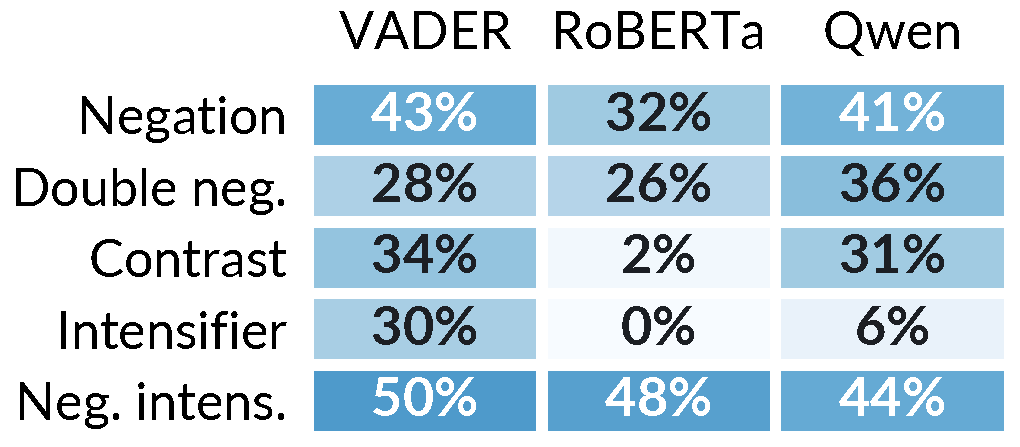
\includegraphics[width=\linewidth]{fig_heatmap.pdf}
\caption{Error rate per phenomenon (\% wrong).}
\end{figure}

\begin{figure}
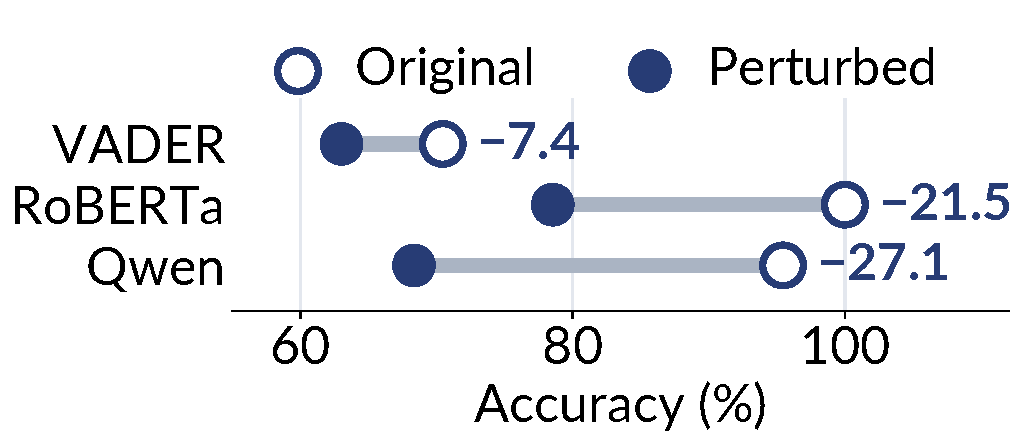
\includegraphics[width=\linewidth]{fig_dumbbell.pdf}
\caption{Accuracy drop from seed to perturbed. The 95\% CI of the drop excludes zero for RoBERTa and Qwen, but not for VADER.}
\end{figure}

\end{block}

\begin{keyblock}{Discussion \& Conclusion}
\textbf{H1} is supported only in absolute terms: while VADER performs weakest overall, its drop of 7.4 points is the \emph{smallest} and not statistically significant --- likely because it begins at just 70.5\% accuracy on the original seeds and thus has less ground to lose. Neither \textbf{H2} nor \textbf{H3} is upheld: RoBERTa fails on \emph{simple} negation as often as on double negation, and the instruction-tuned LLM proves to be the \emph{least} robust, with a decrease of 27.1 points.

RoBERTa achieves perfect accuracy on all seeds but still suffers a 21.5-point loss, with 74\% of its mistakes mirroring the seed's label: high benchmark accuracy does \textbf{not} guarantee compositional understanding (RQ3).

\textbf{Limitations} include testing only English, a single LLM size, and seeds selected for clear polarity.
\end{keyblock}

\begin{exampleblock}{Reproducibility}
Code, test suite, prompts and raw predictions are in our repository (QR code, top right). The models ran in under an hour on one free Colab T4; random seed 42.
\end{exampleblock}

\end{column}
\separatorcolumn
\end{columns}

% ==================== REFERENCES STRIP ====================
\vspace{-1.15cm}
\begin{columns}[t]
\separatorcolumn
\begin{column}{\dimexpr\paperwidth-2\sepwidth\relax}
{\color{navy}\rule{\linewidth}{2pt}}\par\smallskip
{\color{navy}\textbf{References}}\par
\begin{minipage}[t]{0.325\linewidth}\raggedright
\bibent{1}{Ribeiro et al. (2020). Beyond Accuracy: Behavioral Testing of NLP Models with CheckList. \emph{ACL}.}
\bibent{2}{Hossain et al. (2020). An Analysis of Natural Language Inference Benchmarks through the Lens of Negation. \emph{EMNLP}.}
\end{minipage}\hfill
\begin{minipage}[t]{0.325\linewidth}\raggedright
\bibent{3}{Kassner \& Sch\"utze (2020). Negated and Misprimed Probes for Pretrained Language Models. \emph{ACL}.}
\bibent{4}{Hutto \& Gilbert (2014). VADER: A Parsimonious Rule-based Model for Sentiment Analysis. \emph{ICWSM}.}
\end{minipage}\hfill
\begin{minipage}[t]{0.325\linewidth}\raggedright
\bibent{5}{Socher et al. (2013). Recursive Deep Models for Semantic Compositionality over a Sentiment Treebank. \emph{EMNLP}.}
\bibent{6}{Truong et al. (2023). Language Models are not Naysayers: an Analysis of Language Models on Negation. \emph{*SEM}.}
\end{minipage}
\end{column}
\separatorcolumn
\end{columns}

\end{frame}
\end{document}
